\documentclass{standalone}
\usepackage{tikz}
\usetikzlibrary{patterns, positioning}


\begin{document}
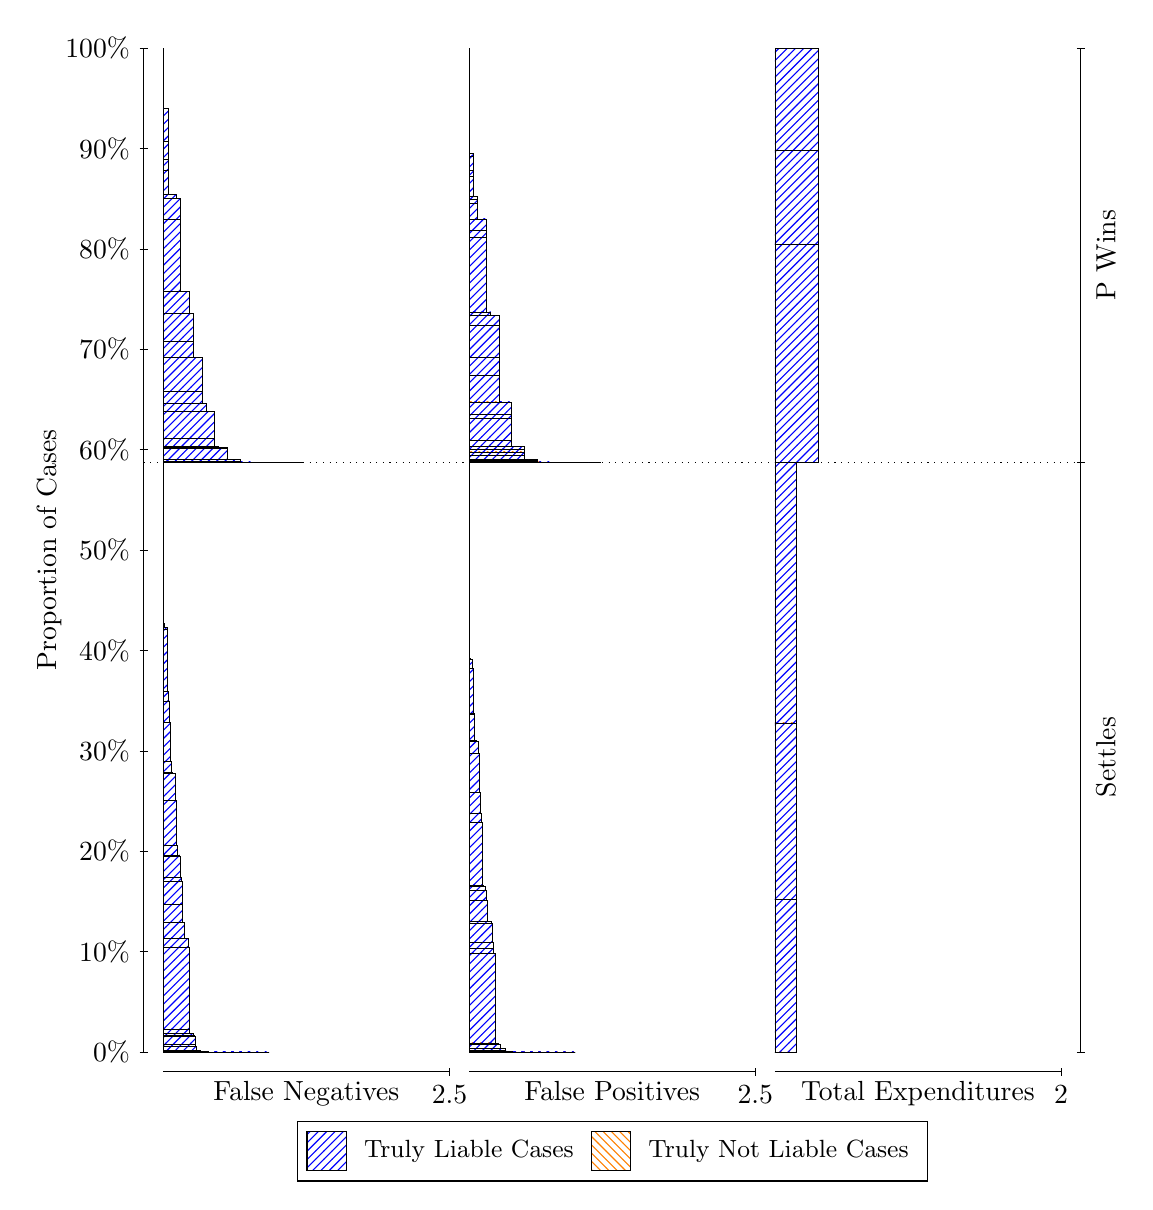
\begin{tikzpicture}
\draw[black, very thin] (1.5,1.75) -- (1.5,14.5);
\node[rotate=90, text=black, anchor=center] at (0.3, 8.125) {Proportion of Cases};
\draw[black, very thin] (1.45,1.75) -- (1.55,1.75);
\node[text=black, anchor=east] at (1.45, 1.75) {0\%};
\draw[black, very thin] (1.45,3.025) -- (1.55,3.025);
\node[text=black, anchor=east] at (1.45, 3.025) {10\%};
\draw[black, very thin] (1.45,4.3) -- (1.55,4.3);
\node[text=black, anchor=east] at (1.45, 4.3) {20\%};
\draw[black, very thin] (1.45,5.575) -- (1.55,5.575);
\node[text=black, anchor=east] at (1.45, 5.575) {30\%};
\draw[black, very thin] (1.45,6.85) -- (1.55,6.85);
\node[text=black, anchor=east] at (1.45, 6.85) {40\%};
\draw[black, very thin] (1.45,8.125) -- (1.55,8.125);
\node[text=black, anchor=east] at (1.45, 8.125) {50\%};
\draw[black, very thin] (1.45,9.4) -- (1.55,9.4);
\node[text=black, anchor=east] at (1.45, 9.4) {60\%};
\draw[black, very thin] (1.45,10.675) -- (1.55,10.675);
\node[text=black, anchor=east] at (1.45, 10.675) {70\%};
\draw[black, very thin] (1.45,11.95) -- (1.55,11.95);
\node[text=black, anchor=east] at (1.45, 11.95) {80\%};
\draw[black, very thin] (1.45,13.225) -- (1.55,13.225);
\node[text=black, anchor=east] at (1.45, 13.225) {90\%};
\draw[black, very thin] (1.45,14.5) -- (1.55,14.5);
\node[text=black, anchor=east] at (1.45, 14.5) {100\%};

\draw[black, very thin] (13.4,1.75) -- (13.4,14.5);
\draw[black, very thin] (13.35,1.75) -- (13.45,1.75);
\node[anchor=west] at (13.35, 1.75) {};
\draw[black, very thin] (13.35,9.2404) -- (13.45,9.2404);
\node[anchor=west] at (13.35, 9.2404) {};
\draw[black, very thin] (13.35,14.5) -- (13.45,14.5);
\node[anchor=west] at (13.35, 14.5) {};

\draw[black, very thin, pattern color=blue, pattern=north east lines] (1.75,1.75) rectangle (3.0943,1.75);
\draw[black, very thin, pattern color=blue, pattern=north east lines] (1.75,1.75) rectangle (2.949,1.75);
\draw[black, very thin, pattern color=blue, pattern=north east lines] (1.75,1.75) rectangle (2.9329,1.75);
\draw[black, very thin, pattern color=blue, pattern=north east lines] (1.75,1.75) rectangle (2.8763,1.75);
\draw[black, very thin, pattern color=blue, pattern=north east lines] (1.75,1.75) rectangle (2.8037,1.75);
\draw[black, very thin, pattern color=blue, pattern=north east lines] (1.75,1.75) rectangle (2.7875,1.75);
\draw[black, very thin, pattern color=blue, pattern=north east lines] (1.75,1.75) rectangle (2.7714,1.75);
\draw[black, very thin, pattern color=blue, pattern=north east lines] (1.75,1.75) rectangle (2.731,1.75);
\draw[black, very thin, pattern color=blue, pattern=north east lines] (1.75,1.75) rectangle (2.7149,1.75);
\draw[black, very thin, pattern color=blue, pattern=north east lines] (1.75,1.75) rectangle (2.6583,1.75);
\draw[black, very thin, pattern color=blue, pattern=north east lines] (1.75,1.75) rectangle (2.6422,1.75);
\draw[black, very thin, pattern color=blue, pattern=north east lines] (1.75,1.75) rectangle (2.626,1.75);
\draw[black, very thin, pattern color=blue, pattern=north east lines] (1.75,1.75) rectangle (2.6099,1.75);
\draw[black, very thin, pattern color=blue, pattern=north east lines] (1.75,1.75) rectangle (2.5857,1.75);
\draw[black, very thin, pattern color=blue, pattern=north east lines] (1.75,1.75) rectangle (2.5695,1.75);
\draw[black, very thin, pattern color=blue, pattern=north east lines] (1.75,1.75) rectangle (2.5534,1.75);
\draw[black, very thin, pattern color=blue, pattern=north east lines] (1.75,1.75) rectangle (2.513,1.75);
\draw[black, very thin, pattern color=blue, pattern=north east lines] (1.75,1.75) rectangle (2.4969,1.75);
\draw[black, very thin, pattern color=blue, pattern=north east lines] (1.75,1.75) rectangle (2.4807,1.75);
\draw[black, very thin, pattern color=blue, pattern=north east lines] (1.75,1.75) rectangle (2.4646,1.75);
\draw[black, very thin, pattern color=blue, pattern=north east lines] (1.75,1.75) rectangle (2.4484,1.75);
\draw[black, very thin, pattern color=blue, pattern=north east lines] (1.75,1.75) rectangle (2.4403,1.75);
\draw[black, very thin, pattern color=blue, pattern=north east lines] (1.75,1.75) rectangle (2.4242,1.75);
\draw[black, very thin, pattern color=blue, pattern=north east lines] (1.75,1.75) rectangle (2.408,1.7501);
\draw[black, very thin, pattern color=blue, pattern=north east lines] (1.75,1.7501) rectangle (2.3919,1.7501);
\draw[black, very thin, pattern color=blue, pattern=north east lines] (1.75,1.7501) rectangle (2.3677,1.7501);
\draw[black, very thin, pattern color=blue, pattern=north east lines] (1.75,1.7501) rectangle (2.3515,1.7501);
\draw[black, very thin, pattern color=blue, pattern=north east lines] (1.75,1.7501) rectangle (2.3354,1.7525);
\draw[black, very thin, pattern color=blue, pattern=north east lines] (1.75,1.7525) rectangle (2.3192,1.753);
\draw[black, very thin, pattern color=blue, pattern=north east lines] (1.75,1.753) rectangle (2.3031,1.7531);
\draw[black, very thin, pattern color=blue, pattern=north east lines] (1.75,1.7531) rectangle (2.2869,1.7536);
\draw[black, very thin, pattern color=blue, pattern=north east lines] (1.75,1.7536) rectangle (2.2789,1.7537);
\draw[black, very thin, pattern color=blue, pattern=north east lines] (1.75,1.7537) rectangle (2.2627,1.7537);
\draw[black, very thin, pattern color=blue, pattern=north east lines] (1.75,1.7537) rectangle (2.2466,1.7586);
\draw[black, very thin, pattern color=blue, pattern=north east lines] (1.75,1.7586) rectangle (2.2304,1.7588);
\draw[black, very thin, pattern color=blue, pattern=north east lines] (1.75,1.7588) rectangle (2.2223,1.7696);
\draw[black, very thin, pattern color=blue, pattern=north east lines] (1.75,1.7696) rectangle (2.2062,1.7698);
\draw[black, very thin, pattern color=blue, pattern=north east lines] (1.75,1.7698) rectangle (2.19,1.7699);
\draw[black, very thin, pattern color=blue, pattern=north east lines] (1.75,1.7699) rectangle (2.1739,1.8182);
\draw[black, very thin, pattern color=blue, pattern=north east lines] (1.75,1.8182) rectangle (2.1577,1.8439);
\draw[black, very thin, pattern color=blue, pattern=north east lines] (1.75,1.8439) rectangle (2.1497,1.9552);
\draw[black, very thin, pattern color=blue, pattern=north east lines] (1.75,1.9552) rectangle (2.1416,1.9601);
\draw[black, very thin, pattern color=blue, pattern=north east lines] (1.75,1.9601) rectangle (2.1254,1.9863);
\draw[black, very thin, pattern color=blue, pattern=north east lines] (1.75,1.9863) rectangle (2.1174,1.9893);
\draw[black, very thin, pattern color=blue, pattern=north east lines] (1.75,1.9893) rectangle (2.1012,1.9893);
\draw[black, very thin, pattern color=blue, pattern=north east lines] (1.75,1.9893) rectangle (2.0851,2.0424);
\draw[black, very thin, pattern color=blue, pattern=north east lines] (1.75,2.0424) rectangle (2.077,3.0829);
\draw[black, very thin, pattern color=blue, pattern=north east lines] (1.75,3.0829) rectangle (2.0689,3.0853);
\draw[black, very thin, pattern color=blue, pattern=north east lines] (1.75,3.0853) rectangle (2.0609,3.1944);
\draw[black, very thin, pattern color=blue, pattern=north east lines] (1.75,3.1944) rectangle (2.0447,3.1967);
\draw[black, very thin, pattern color=blue, pattern=north east lines] (1.75,3.1967) rectangle (2.0286,3.1987);
\draw[black, very thin, pattern color=blue, pattern=north east lines] (1.75,3.1987) rectangle (2.0124,3.3912);
\draw[black, very thin, pattern color=blue, pattern=north east lines] (1.75,3.3912) rectangle (1.9963,3.632);
\draw[black, very thin, pattern color=blue, pattern=north east lines] (1.75,3.632) rectangle (1.9882,3.914);
\draw[black, very thin, pattern color=blue, pattern=north east lines] (1.75,3.914) rectangle (1.9801,3.967);
\draw[black, very thin, pattern color=blue, pattern=north east lines] (1.75,3.967) rectangle (1.964,4.2345);
\draw[black, very thin, pattern color=blue, pattern=north east lines] (1.75,4.2345) rectangle (1.9559,4.2537);
\draw[black, very thin, pattern color=blue, pattern=north east lines] (1.75,4.2537) rectangle (1.9397,4.2537);
\draw[black, very thin, pattern color=blue, pattern=north east lines] (1.75,4.2537) rectangle (1.9236,4.3702);
\draw[black, very thin, pattern color=blue, pattern=north east lines] (1.75,4.3702) rectangle (1.9155,4.9415);
\draw[black, very thin, pattern color=blue, pattern=north east lines] (1.75,4.9415) rectangle (1.9074,4.9472);
\draw[black, very thin, pattern color=blue, pattern=north east lines] (1.75,4.9472) rectangle (1.8994,5.2859);
\draw[black, very thin, pattern color=blue, pattern=north east lines] (1.75,5.2859) rectangle (1.8832,5.2911);
\draw[black, very thin, pattern color=blue, pattern=north east lines] (1.75,5.2911) rectangle (1.8671,5.2962);
\draw[black, very thin, pattern color=blue, pattern=north east lines] (1.75,5.2962) rectangle (1.8509,5.4439);
\draw[black, very thin, pattern color=blue, pattern=north east lines] (1.75,5.4439) rectangle (1.8348,5.9416);
\draw[black, very thin, pattern color=blue, pattern=north east lines] (1.75,5.9416) rectangle (1.8267,6.2091);
\draw[black, very thin, pattern color=blue, pattern=north east lines] (1.75,6.2091) rectangle (1.8186,6.327);
\draw[black, very thin, pattern color=blue, pattern=north east lines] (1.75,6.327) rectangle (1.8025,7.1194);
\draw[black, very thin, pattern color=blue, pattern=north east lines] (1.75,7.1194) rectangle (1.7944,7.1386);
\draw[black, very thin, pattern color=blue, pattern=north east lines] (1.75,7.1386) rectangle (1.7783,7.1386);
\draw[black, very thin, pattern color=blue, pattern=north east lines] (1.75,7.1386) rectangle (1.7621,7.1917);
\draw[black, very thin, pattern color=blue, pattern=north east lines] (1.75,7.1917) rectangle (1.754,7.3097);
\draw[black, very thin, pattern color=orange, pattern=north west lines] (1.75,7.3097) rectangle (1.75,7.3097);
\draw[black, very thin, pattern color=blue, pattern=north east lines] (1.75,7.3097) rectangle (1.75,9.2404);
\draw[black, very thin, pattern color=blue, pattern=north east lines] (1.75,9.2404) rectangle (3.5303,9.2404);
\draw[black, very thin, pattern color=blue, pattern=north east lines] (1.75,9.2404) rectangle (3.3689,9.2404);
\draw[black, very thin, pattern color=blue, pattern=north east lines] (1.75,9.2404) rectangle (3.2074,9.2404);
\draw[black, very thin, pattern color=blue, pattern=north east lines] (1.75,9.2404) rectangle (3.0984,9.2404);
\draw[black, very thin, pattern color=blue, pattern=north east lines] (1.75,9.2404) rectangle (3.0459,9.2406);
\draw[black, very thin, pattern color=blue, pattern=north east lines] (1.75,9.2406) rectangle (2.9369,9.2406);
\draw[black, very thin, pattern color=blue, pattern=north east lines] (1.75,9.2406) rectangle (2.8844,9.2426);
\draw[black, very thin, pattern color=blue, pattern=north east lines] (1.75,9.2426) rectangle (2.8844,9.2442);
\draw[black, very thin, pattern color=blue, pattern=north east lines] (1.75,9.2442) rectangle (2.7754,9.2442);
\draw[black, very thin, pattern color=blue, pattern=north east lines] (1.75,9.2442) rectangle (2.7754,9.2442);
\draw[black, very thin, pattern color=blue, pattern=north east lines] (1.75,9.2442) rectangle (2.7229,9.2568);
\draw[black, very thin, pattern color=blue, pattern=north east lines] (1.75,9.2568) rectangle (2.7229,9.2749);
\draw[black, very thin, pattern color=blue, pattern=north east lines] (1.75,9.2749) rectangle (2.6139,9.2751);
\draw[black, very thin, pattern color=blue, pattern=north east lines] (1.75,9.2751) rectangle (2.5614,9.4221);
\draw[black, very thin, pattern color=blue, pattern=north east lines] (1.75,9.4221) rectangle (2.5614,9.432);
\draw[black, very thin, pattern color=blue, pattern=north east lines] (1.75,9.432) rectangle (2.4524,9.4334);
\draw[black, very thin, pattern color=blue, pattern=north east lines] (1.75,9.4334) rectangle (2.4524,9.4375);
\draw[black, very thin, pattern color=blue, pattern=north east lines] (1.75,9.4375) rectangle (2.4,9.5386);
\draw[black, very thin, pattern color=blue, pattern=north east lines] (1.75,9.5386) rectangle (2.4,9.8885);
\draw[black, very thin, pattern color=blue, pattern=north east lines] (1.75,9.8885) rectangle (2.291,9.9859);
\draw[black, very thin, pattern color=blue, pattern=north east lines] (1.75,9.9859) rectangle (2.2385,10.135);
\draw[black, very thin, pattern color=blue, pattern=north east lines] (1.75,10.135) rectangle (2.2385,10.57);
\draw[black, very thin, pattern color=blue, pattern=north east lines] (1.75,10.57) rectangle (2.2385,10.574);
\draw[black, very thin, pattern color=blue, pattern=north east lines] (1.75,10.574) rectangle (2.1295,10.776);
\draw[black, very thin, pattern color=blue, pattern=north east lines] (1.75,10.776) rectangle (2.1295,11.127);
\draw[black, very thin, pattern color=blue, pattern=north east lines] (1.75,11.127) rectangle (2.077,11.409);
\draw[black, very thin, pattern color=blue, pattern=north east lines] (1.75,11.409) rectangle (1.968,12.326);
\draw[black, very thin, pattern color=blue, pattern=north east lines] (1.75,12.326) rectangle (1.968,12.591);
\draw[black, very thin, pattern color=blue, pattern=north east lines] (1.75,12.591) rectangle (1.9155,12.591);
\draw[black, very thin, pattern color=blue, pattern=north east lines] (1.75,12.591) rectangle (1.9155,12.639);
\draw[black, very thin, pattern color=blue, pattern=north east lines] (1.75,12.639) rectangle (1.9155,12.639);
\draw[black, very thin, pattern color=blue, pattern=north east lines] (1.75,12.639) rectangle (1.8065,12.953);
\draw[black, very thin, pattern color=blue, pattern=north east lines] (1.75,12.953) rectangle (1.8065,13.083);
\draw[black, very thin, pattern color=blue, pattern=north east lines] (1.75,13.083) rectangle (1.8065,13.317);
\draw[black, very thin, pattern color=blue, pattern=north east lines] (1.75,13.317) rectangle (1.8065,13.735);
\draw[black, very thin, pattern color=blue, pattern=north east lines] (1.75,13.735) rectangle (1.754,13.735);
\draw[black, very thin, pattern color=blue, pattern=north east lines] (1.75,13.735) rectangle (1.754,13.735);
\draw[black, very thin, pattern color=orange, pattern=north west lines] (1.75,13.735) rectangle (1.75,13.735);
\draw[black, very thin, pattern color=blue, pattern=north east lines] (1.75,13.735) rectangle (1.75,14.5);
\draw[black, very thin, pattern color=orange, pattern=north west lines] (5.6333,1.75) rectangle (6.9777,1.75);
\draw[black, very thin, pattern color=blue, pattern=north east lines] (5.6333,1.75) rectangle (6.9777,1.75);
\draw[black, very thin, pattern color=orange, pattern=north west lines] (5.6333,1.75) rectangle (6.905,1.75);
\draw[black, very thin, pattern color=blue, pattern=north east lines] (5.6333,1.75) rectangle (6.905,1.75);
\draw[black, very thin, pattern color=orange, pattern=north west lines] (5.6333,1.75) rectangle (6.8323,1.75);
\draw[black, very thin, pattern color=blue, pattern=north east lines] (5.6333,1.75) rectangle (6.8323,1.75);
\draw[black, very thin, pattern color=blue, pattern=north east lines] (5.6333,1.75) rectangle (6.8162,1.75);
\draw[black, very thin, pattern color=blue, pattern=north east lines] (5.6333,1.75) rectangle (6.7435,1.75);
\draw[black, very thin, pattern color=orange, pattern=north west lines] (5.6333,1.75) rectangle (6.687,1.75);
\draw[black, very thin, pattern color=blue, pattern=north east lines] (5.6333,1.75) rectangle (6.687,1.75);
\draw[black, very thin, pattern color=blue, pattern=north east lines] (5.6333,1.75) rectangle (6.6709,1.75);
\draw[black, very thin, pattern color=blue, pattern=north east lines] (5.6333,1.75) rectangle (6.6547,1.75);
\draw[black, very thin, pattern color=orange, pattern=north west lines] (5.6333,1.75) rectangle (6.6143,1.75);
\draw[black, very thin, pattern color=blue, pattern=north east lines] (5.6333,1.75) rectangle (6.6143,1.75);
\draw[black, very thin, pattern color=blue, pattern=north east lines] (5.6333,1.75) rectangle (6.582,1.75);
\draw[black, very thin, pattern color=orange, pattern=north west lines] (5.6333,1.75) rectangle (6.5417,1.75);
\draw[black, very thin, pattern color=blue, pattern=north east lines] (5.6333,1.75) rectangle (6.5417,1.75);
\draw[black, very thin, pattern color=blue, pattern=north east lines] (5.6333,1.75) rectangle (6.5255,1.75);
\draw[black, very thin, pattern color=blue, pattern=north east lines] (5.6333,1.75) rectangle (6.5094,1.75);
\draw[black, very thin, pattern color=blue, pattern=north east lines] (5.6333,1.75) rectangle (6.4932,1.75);
\draw[black, very thin, pattern color=orange, pattern=north west lines] (5.6333,1.75) rectangle (6.469,1.75);
\draw[black, very thin, pattern color=blue, pattern=north east lines] (5.6333,1.75) rectangle (6.469,1.75);
\draw[black, very thin, pattern color=blue, pattern=north east lines] (5.6333,1.75) rectangle (6.4529,1.75);
\draw[black, very thin, pattern color=blue, pattern=north east lines] (5.6333,1.75) rectangle (6.4206,1.75);
\draw[black, very thin, pattern color=orange, pattern=north west lines] (5.6333,1.75) rectangle (6.3963,1.75);
\draw[black, very thin, pattern color=blue, pattern=north east lines] (5.6333,1.75) rectangle (6.3963,1.75);
\draw[black, very thin, pattern color=blue, pattern=north east lines] (5.6333,1.75) rectangle (6.3802,1.75);
\draw[black, very thin, pattern color=blue, pattern=north east lines] (5.6333,1.75) rectangle (6.364,1.75);
\draw[black, very thin, pattern color=blue, pattern=north east lines] (5.6333,1.75) rectangle (6.3479,1.75);
\draw[black, very thin, pattern color=blue, pattern=north east lines] (5.6333,1.75) rectangle (6.3317,1.75);
\draw[black, very thin, pattern color=orange, pattern=north west lines] (5.6333,1.75) rectangle (6.3237,1.75);
\draw[black, very thin, pattern color=blue, pattern=north east lines] (5.6333,1.75) rectangle (6.3237,1.75);
\draw[black, very thin, pattern color=blue, pattern=north east lines] (5.6333,1.75) rectangle (6.3075,1.75);
\draw[black, very thin, pattern color=blue, pattern=north east lines] (5.6333,1.75) rectangle (6.2914,1.75);
\draw[black, very thin, pattern color=blue, pattern=north east lines] (5.6333,1.75) rectangle (6.2591,1.7501);
\draw[black, very thin, pattern color=orange, pattern=north west lines] (5.6333,1.7501) rectangle (6.251,1.7501);
\draw[black, very thin, pattern color=blue, pattern=north east lines] (5.6333,1.7501) rectangle (6.251,1.7512);
\draw[black, very thin, pattern color=blue, pattern=north east lines] (5.6333,1.7512) rectangle (6.2349,1.7512);
\draw[black, very thin, pattern color=blue, pattern=north east lines] (5.6333,1.7512) rectangle (6.2187,1.7512);
\draw[black, very thin, pattern color=blue, pattern=north east lines] (5.6333,1.7512) rectangle (6.2026,1.7512);
\draw[black, very thin, pattern color=blue, pattern=north east lines] (5.6333,1.7512) rectangle (6.1864,1.7536);
\draw[black, very thin, pattern color=orange, pattern=north west lines] (5.6333,1.7536) rectangle (6.1783,1.7536);
\draw[black, very thin, pattern color=blue, pattern=north east lines] (5.6333,1.7536) rectangle (6.1783,1.7536);
\draw[black, very thin, pattern color=blue, pattern=north east lines] (5.6333,1.7536) rectangle (6.1703,1.7536);
\draw[black, very thin, pattern color=blue, pattern=north east lines] (5.6333,1.7536) rectangle (6.1622,1.7537);
\draw[black, very thin, pattern color=blue, pattern=north east lines] (5.6333,1.7537) rectangle (6.146,1.7537);
\draw[black, very thin, pattern color=blue, pattern=north east lines] (5.6333,1.7537) rectangle (6.1299,1.7538);
\draw[black, very thin, pattern color=orange, pattern=north west lines] (5.6333,1.7538) rectangle (6.1057,1.7538);
\draw[black, very thin, pattern color=blue, pattern=north east lines] (5.6333,1.7538) rectangle (6.1057,1.7641);
\draw[black, very thin, pattern color=blue, pattern=north east lines] (5.6333,1.7641) rectangle (6.0976,1.7696);
\draw[black, very thin, pattern color=blue, pattern=north east lines] (5.6333,1.7696) rectangle (6.0895,1.799);
\draw[black, very thin, pattern color=blue, pattern=north east lines] (5.6333,1.799) rectangle (6.0734,1.7995);
\draw[black, very thin, pattern color=blue, pattern=north east lines] (5.6333,1.7995) rectangle (6.0572,1.7997);
\draw[black, very thin, pattern color=blue, pattern=north east lines] (5.6333,1.7997) rectangle (6.0411,1.7998);
\draw[black, very thin, pattern color=blue, pattern=north east lines] (5.6333,1.7998) rectangle (6.0249,1.8528);
\draw[black, very thin, pattern color=blue, pattern=north east lines] (5.6333,1.8528) rectangle (6.0169,1.853);
\draw[black, very thin, pattern color=blue, pattern=north east lines] (5.6333,1.853) rectangle (6.0088,1.8586);
\draw[black, very thin, pattern color=blue, pattern=north east lines] (5.6333,1.8586) rectangle (6.0007,1.8636);
\draw[black, very thin, pattern color=blue, pattern=north east lines] (5.6333,1.8636) rectangle (5.9846,1.8636);
\draw[black, very thin, pattern color=blue, pattern=north east lines] (5.6333,1.8636) rectangle (5.9684,1.8666);
\draw[black, very thin, pattern color=orange, pattern=north west lines] (5.6333,1.8666) rectangle (5.9603,1.8666);
\draw[black, very thin, pattern color=blue, pattern=north east lines] (5.6333,1.8666) rectangle (5.9603,3.0081);
\draw[black, very thin, pattern color=blue, pattern=north east lines] (5.6333,3.0081) rectangle (5.9442,3.069);
\draw[black, very thin, pattern color=blue, pattern=north east lines] (5.6333,3.069) rectangle (5.9361,3.1426);
\draw[black, very thin, pattern color=blue, pattern=north east lines] (5.6333,3.1426) rectangle (5.928,3.3864);
\draw[black, very thin, pattern color=blue, pattern=north east lines] (5.6333,3.3864) rectangle (5.9119,3.4069);
\draw[black, very thin, pattern color=blue, pattern=north east lines] (5.6333,3.4069) rectangle (5.8957,3.4092);
\draw[black, very thin, pattern color=blue, pattern=north east lines] (5.6333,3.4092) rectangle (5.8796,3.4111);
\draw[black, very thin, pattern color=blue, pattern=north east lines] (5.6333,3.4111) rectangle (5.8634,3.6783);
\draw[black, very thin, pattern color=blue, pattern=north east lines] (5.6333,3.6783) rectangle (5.8554,3.6807);
\draw[black, very thin, pattern color=blue, pattern=north east lines] (5.6333,3.6807) rectangle (5.8473,3.7987);
\draw[black, very thin, pattern color=blue, pattern=north east lines] (5.6333,3.7987) rectangle (5.8392,3.8517);
\draw[black, very thin, pattern color=blue, pattern=north east lines] (5.6333,3.8517) rectangle (5.8231,3.8518);
\draw[black, very thin, pattern color=blue, pattern=north east lines] (5.6333,3.8518) rectangle (5.8069,3.871);
\draw[black, very thin, pattern color=blue, pattern=north east lines] (5.6333,3.871) rectangle (5.7989,4.6633);
\draw[black, very thin, pattern color=blue, pattern=north east lines] (5.6333,4.6633) rectangle (5.7827,4.7813);
\draw[black, very thin, pattern color=blue, pattern=north east lines] (5.6333,4.7813) rectangle (5.7746,5.0488);
\draw[black, very thin, pattern color=blue, pattern=north east lines] (5.6333,5.0488) rectangle (5.7666,5.5465);
\draw[black, very thin, pattern color=blue, pattern=north east lines] (5.6333,5.5465) rectangle (5.7504,5.6941);
\draw[black, very thin, pattern color=blue, pattern=north east lines] (5.6333,5.6941) rectangle (5.7343,5.6993);
\draw[black, very thin, pattern color=blue, pattern=north east lines] (5.6333,5.6993) rectangle (5.7181,5.7044);
\draw[black, very thin, pattern color=blue, pattern=north east lines] (5.6333,5.7044) rectangle (5.702,6.0432);
\draw[black, very thin, pattern color=blue, pattern=north east lines] (5.6333,6.0432) rectangle (5.6939,6.0488);
\draw[black, very thin, pattern color=blue, pattern=north east lines] (5.6333,6.0488) rectangle (5.6858,6.6201);
\draw[black, very thin, pattern color=blue, pattern=north east lines] (5.6333,6.6201) rectangle (5.6777,6.7367);
\draw[black, very thin, pattern color=blue, pattern=north east lines] (5.6333,6.7367) rectangle (5.6616,6.7367);
\draw[black, very thin, pattern color=blue, pattern=north east lines] (5.6333,6.7367) rectangle (5.6454,6.7559);
\draw[black, very thin, pattern color=blue, pattern=north east lines] (5.6333,6.7559) rectangle (5.6374,7.0234);
\draw[black, very thin, pattern color=blue, pattern=north east lines] (5.6333,7.0234) rectangle (5.6333,9.2404);
\draw[black, very thin, pattern color=orange, pattern=north west lines] (5.6333,9.2404) rectangle (7.3047,9.2404);
\draw[black, very thin, pattern color=blue, pattern=north east lines] (5.6333,9.2404) rectangle (7.3047,9.2404);
\draw[black, very thin, pattern color=orange, pattern=north west lines] (5.6333,9.2404) rectangle (7.1432,9.2404);
\draw[black, very thin, pattern color=blue, pattern=north east lines] (5.6333,9.2404) rectangle (7.1432,9.2404);
\draw[black, very thin, pattern color=orange, pattern=north west lines] (5.6333,9.2404) rectangle (6.9817,9.2404);
\draw[black, very thin, pattern color=blue, pattern=north east lines] (5.6333,9.2404) rectangle (6.9817,9.2404);
\draw[black, very thin, pattern color=blue, pattern=north east lines] (5.6333,9.2404) rectangle (6.9817,9.2404);
\draw[black, very thin, pattern color=blue, pattern=north east lines] (5.6333,9.2404) rectangle (6.9817,9.2404);
\draw[black, very thin, pattern color=orange, pattern=north west lines] (5.6333,9.2404) rectangle (6.8202,9.2404);
\draw[black, very thin, pattern color=blue, pattern=north east lines] (5.6333,9.2404) rectangle (6.8202,9.2405);
\draw[black, very thin, pattern color=blue, pattern=north east lines] (5.6333,9.2405) rectangle (6.8202,9.2406);
\draw[black, very thin, pattern color=orange, pattern=north west lines] (5.6333,9.2406) rectangle (6.7112,9.2406);
\draw[black, very thin, pattern color=blue, pattern=north east lines] (5.6333,9.2406) rectangle (6.7112,9.2406);
\draw[black, very thin, pattern color=orange, pattern=north west lines] (5.6333,9.2406) rectangle (6.6587,9.2406);
\draw[black, very thin, pattern color=blue, pattern=north east lines] (5.6333,9.2406) rectangle (6.6587,9.2417);
\draw[black, very thin, pattern color=blue, pattern=north east lines] (5.6333,9.2417) rectangle (6.6587,9.2439);
\draw[black, very thin, pattern color=orange, pattern=north west lines] (5.6333,9.2439) rectangle (6.5497,9.2439);
\draw[black, very thin, pattern color=blue, pattern=north east lines] (5.6333,9.2439) rectangle (6.5497,9.2439);
\draw[black, very thin, pattern color=blue, pattern=north east lines] (5.6333,9.2439) rectangle (6.4973,9.2532);
\draw[black, very thin, pattern color=orange, pattern=north west lines] (5.6333,9.2532) rectangle (6.4973,9.2532);
\draw[black, very thin, pattern color=blue, pattern=north east lines] (5.6333,9.2532) rectangle (6.4973,9.2605);
\draw[black, very thin, pattern color=blue, pattern=north east lines] (5.6333,9.2605) rectangle (6.4973,9.2746);
\draw[black, very thin, pattern color=orange, pattern=north west lines] (5.6333,9.2746) rectangle (6.3883,9.2746);
\draw[black, very thin, pattern color=blue, pattern=north east lines] (5.6333,9.2746) rectangle (6.3883,9.2746);
\draw[black, very thin, pattern color=blue, pattern=north east lines] (5.6333,9.2746) rectangle (6.3358,9.3288);
\draw[black, very thin, pattern color=blue, pattern=north east lines] (5.6333,9.3288) rectangle (6.3358,9.3702);
\draw[black, very thin, pattern color=orange, pattern=north west lines] (5.6333,9.3702) rectangle (6.3358,9.3702);
\draw[black, very thin, pattern color=blue, pattern=north east lines] (5.6333,9.3702) rectangle (6.3358,9.4101);
\draw[black, very thin, pattern color=blue, pattern=north east lines] (5.6333,9.4101) rectangle (6.3358,9.445);
\draw[black, very thin, pattern color=orange, pattern=north west lines] (5.6333,9.445) rectangle (6.2268,9.445);
\draw[black, very thin, pattern color=blue, pattern=north east lines] (5.6333,9.445) rectangle (6.2268,9.445);
\draw[black, very thin, pattern color=blue, pattern=north east lines] (5.6333,9.445) rectangle (6.2268,9.445);
\draw[black, very thin, pattern color=blue, pattern=north east lines] (5.6333,9.445) rectangle (6.1743,9.5143);
\draw[black, very thin, pattern color=orange, pattern=north west lines] (5.6333,9.5143) rectangle (6.1743,9.5143);
\draw[black, very thin, pattern color=blue, pattern=north east lines] (5.6333,9.5143) rectangle (6.1743,9.7958);
\draw[black, very thin, pattern color=blue, pattern=north east lines] (5.6333,9.7958) rectangle (6.1743,9.8473);
\draw[black, very thin, pattern color=blue, pattern=north east lines] (5.6333,9.8473) rectangle (6.1743,10.006);
\draw[black, very thin, pattern color=orange, pattern=north west lines] (5.6333,10.006) rectangle (6.0653,10.006);
\draw[black, very thin, pattern color=blue, pattern=north east lines] (5.6333,10.006) rectangle (6.0653,10.006);
\draw[black, very thin, pattern color=blue, pattern=north east lines] (5.6333,10.006) rectangle (6.0653,10.006);
\draw[black, very thin, pattern color=blue, pattern=north east lines] (5.6333,10.006) rectangle (6.0128,10.345);
\draw[black, very thin, pattern color=blue, pattern=north east lines] (5.6333,10.345) rectangle (6.0128,10.574);
\draw[black, very thin, pattern color=blue, pattern=north east lines] (5.6333,10.574) rectangle (6.0128,10.982);
\draw[black, very thin, pattern color=blue, pattern=north east lines] (5.6333,10.982) rectangle (6.0128,11.102);
\draw[black, very thin, pattern color=orange, pattern=north west lines] (5.6333,11.102) rectangle (5.9038,11.102);
\draw[black, very thin, pattern color=blue, pattern=north east lines] (5.6333,11.102) rectangle (5.9038,11.148);
\draw[black, very thin, pattern color=blue, pattern=north east lines] (5.6333,11.148) rectangle (5.9038,11.15);
\draw[black, very thin, pattern color=blue, pattern=north east lines] (5.6333,11.15) rectangle (5.9038,11.15);
\draw[black, very thin, pattern color=blue, pattern=north east lines] (5.6333,11.15) rectangle (5.8513,12.091);
\draw[black, very thin, pattern color=blue, pattern=north east lines] (5.6333,12.091) rectangle (5.8513,12.188);
\draw[black, very thin, pattern color=blue, pattern=north east lines] (5.6333,12.188) rectangle (5.8513,12.331);
\draw[black, very thin, pattern color=blue, pattern=north east lines] (5.6333,12.331) rectangle (5.7423,12.526);
\draw[black, very thin, pattern color=orange, pattern=north west lines] (5.6333,12.526) rectangle (5.7423,12.526);
\draw[black, very thin, pattern color=blue, pattern=north east lines] (5.6333,12.526) rectangle (5.7423,12.577);
\draw[black, very thin, pattern color=blue, pattern=north east lines] (5.6333,12.577) rectangle (5.7423,12.614);
\draw[black, very thin, pattern color=blue, pattern=north east lines] (5.6333,12.614) rectangle (5.6899,12.868);
\draw[black, very thin, pattern color=blue, pattern=north east lines] (5.6333,12.868) rectangle (5.6899,12.946);
\draw[black, very thin, pattern color=blue, pattern=north east lines] (5.6333,12.946) rectangle (5.6899,13.129);
\draw[black, very thin, pattern color=blue, pattern=north east lines] (5.6333,13.129) rectangle (5.6899,13.166);
\draw[black, very thin, pattern color=blue, pattern=north east lines] (5.6333,13.166) rectangle (5.6333,14.5);
\draw[black, very thin, pattern color=orange, pattern=north west lines] (9.5167,1.75) rectangle (9.7892,1.75);
\draw[black, very thin, pattern color=blue, pattern=north east lines] (9.5167,1.75) rectangle (9.7892,3.6919);
\draw[black, very thin, pattern color=orange, pattern=north west lines] (9.5167,3.6919) rectangle (9.7892,3.6919);
\draw[black, very thin, pattern color=blue, pattern=north east lines] (9.5167,3.6919) rectangle (9.7892,5.9296);
\draw[black, very thin, pattern color=orange, pattern=north west lines] (9.5167,5.9296) rectangle (9.7892,5.9296);
\draw[black, very thin, pattern color=blue, pattern=north east lines] (9.5167,5.9296) rectangle (9.7892,9.2404);
\draw[black, very thin, pattern color=orange, pattern=north west lines] (9.5167,9.2404) rectangle (10.062,9.2404);
\draw[black, very thin, pattern color=blue, pattern=north east lines] (9.5167,9.2404) rectangle (10.062,12.008);
\draw[black, very thin, pattern color=orange, pattern=north west lines] (9.5167,12.008) rectangle (10.062,12.008);
\draw[black, very thin, pattern color=blue, pattern=north east lines] (9.5167,12.008) rectangle (10.062,13.203);
\draw[black, very thin, pattern color=orange, pattern=north west lines] (9.5167,13.203) rectangle (10.062,13.203);
\draw[black, very thin, pattern color=blue, pattern=north east lines] (9.5167,13.203) rectangle (10.062,14.5);
\draw[black, dotted] (1.5,9.2404) -- (13.4,9.2404);
\draw[black, very thin] (1.75,1.5) -- (5.3833,1.5);
\node[text=black, anchor=north] at (3.5667, 1.5) {False Negatives};
\draw[black, very thin] (5.3833,1.45) -- (5.3833,1.55);
\node[text=black, anchor=north] at (5.3833, 1.45) {2.5};

\draw[black, very thin] (5.6333,1.5) -- (9.2667,1.5);
\node[text=black, anchor=north] at (7.45, 1.5) {False Positives};
\draw[black, very thin] (9.2667,1.45) -- (9.2667,1.55);
\node[text=black, anchor=north] at (9.2667, 1.45) {2.5};

\draw[black, very thin] (9.5167,1.5) -- (13.15,1.5);
\node[text=black, anchor=north] at (11.333, 1.5) {Total Expenditures};
\draw[black, very thin] (13.15,1.45) -- (13.15,1.55);
\node[text=black, anchor=north] at (13.15, 1.45) {2};

\node[text=black, centered, rotate=90] at (13.72, 5.4952) {Settles};
\node[text=black, centered, rotate=90] at (13.72, 11.87) {P Wins};

\draw (7.449999999999999,1.5) node[draw=none] (baseCoordinate) {};
\begin{scope}[align=center]
        \matrix[scale=0.5, draw=black, below=0.5cm of baseCoordinate, nodes={draw}, column sep=0.1cm]{
            \node[rectangle, draw, minimum width=0.5cm, minimum height=0.5cm, pattern color=blue, pattern=north east lines] {}; &
            \node[draw=none, font=\small, text=black] (B) {Truly Liable Cases}; &
            \node[rectangle, draw, minimum width=0.5cm, minimum height=0.5cm, pattern color=orange, pattern=north west lines] {}; &
            \node[draw=none, font=\small, text=black] (B) {Truly Not Liable Cases}; \\
            };
\end{scope}

\end{tikzpicture}
\end{document}